\chapter{Case Study: Snake Game}\label{chap:casestudy}

The first implementation started with a simple \textit{Pong} game that was then split and evolved into the actual game engine. After most of the engine was implemented, we developed a \textit{Snake} game with and without the engine to compare both versions. In this case study, we show the differences between both versions and how the engine makes game development simpler and better organized.

\textit{Snake} is more of a genre than a single game. The first version that was for a single player with one snake that eats apples to grow larger was \textit{Snake Byte} written by Chuck Sommerville for the Apple II and published by Sirius Software in 1982. The player can control the next direction the head of the snake turns to, which moves on a grid. \textit{Snake Byte} was based on 28 levels, whereas our version, like many simple implementations, use just a single apple. For these single level implementations, one apple always exists in the world that adds one score when eating, while also increasing the snake's length by one grid unit. The game is over when the snake head runs into an outer wall or its own tail.\\
Our version is based on this simple single level concept for the most part. A screenshot during the gameplay of this Snake implementation can be seen in \Cref{fig:snake}.

\begin{figure}[h!]
\centering
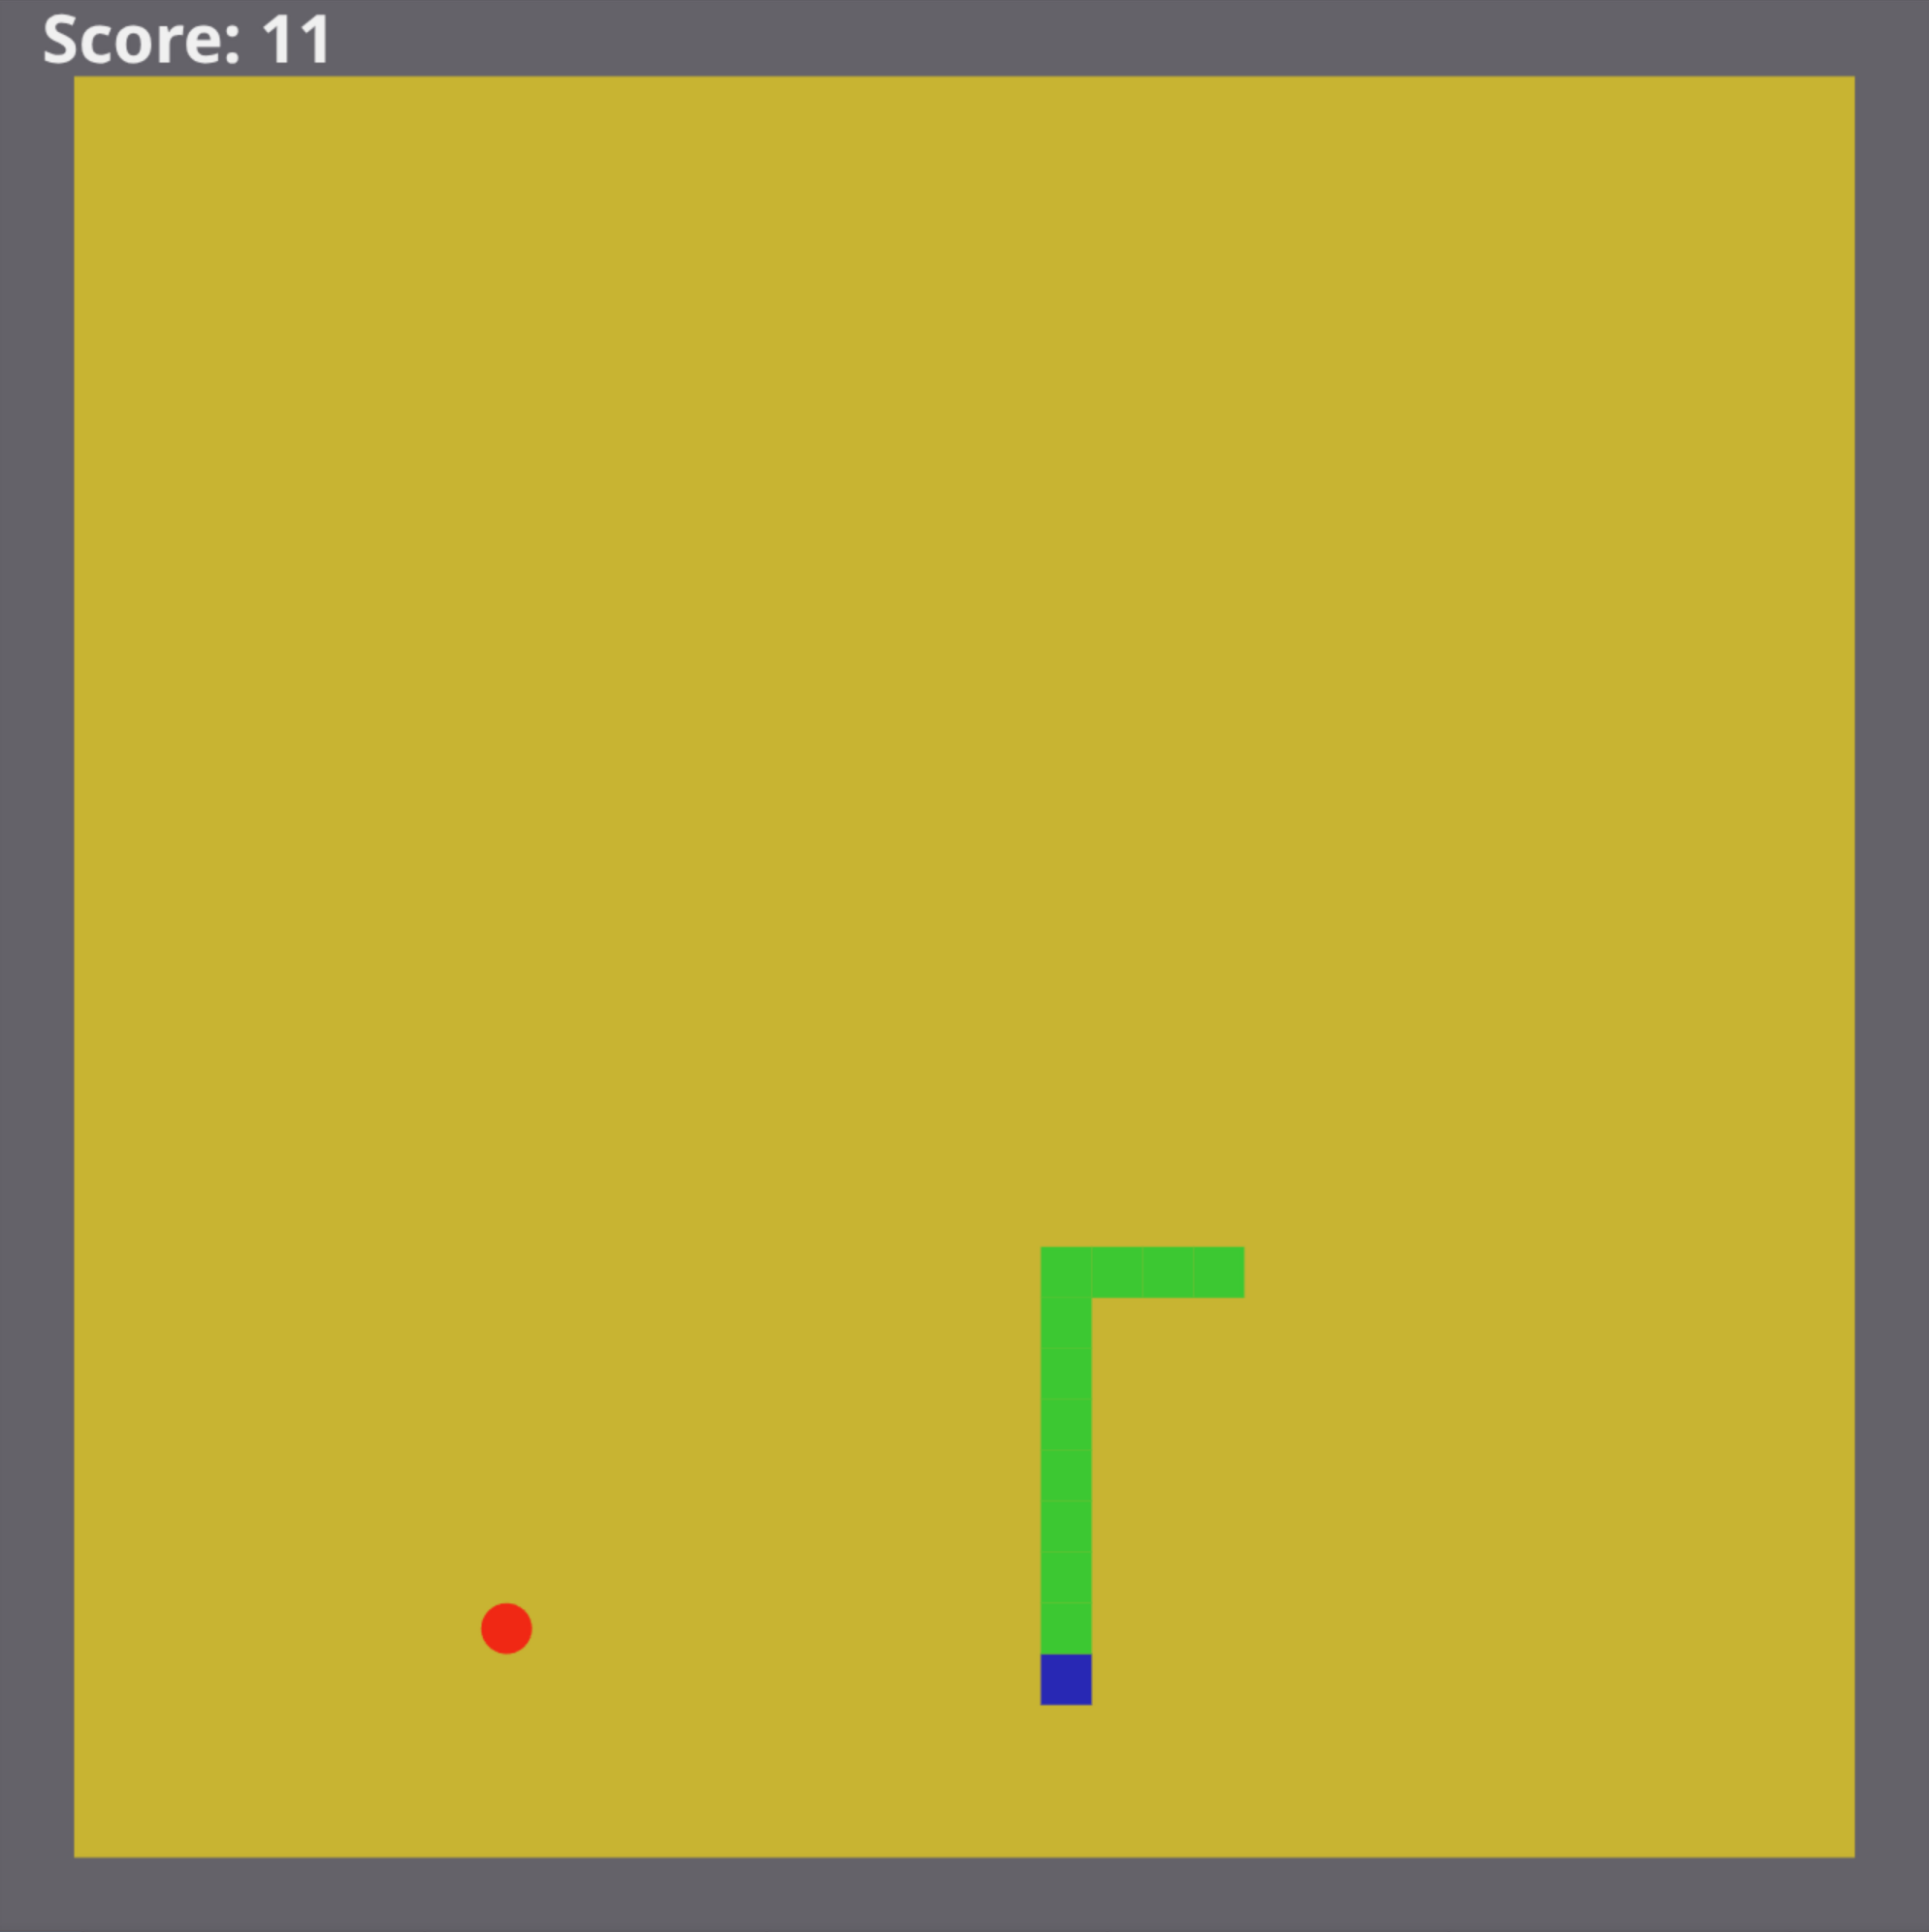
\includegraphics[width=\linewidth]{img/snake_screenshot.png}
\caption{Screenshot of the Snake Game (version using the game engine).}
\label{fig:snake}
\end{figure}

\section{Defining Components and Resources}

For the game engine version, all required components are defined as |records| at the start:

\begin{lstlisting}
record SnakeTag()
record MoveDir(next: Vector2Int, last: Vector2Int)
record LastPosition(value: Vector2)
record NextTail(value: Entity)
record Score(value: Int)
\end{lstlisting}

The components are then registered at the start of the main function after defining the default panicking ECS exception handler and initializing the |engineWorld| and |canvasRenderer|:

\begin{lstlisting}
with panicOnEcsException();

// ECS, engine & renderer init
with engineWorld();
with canvasRenderer();

// Our components
with component[SnakeTag]();
with component[MoveDir]();
...
\end{lstlisting}

The required resources are defined the same way as the components:

\begin{lstlisting}
record GameOver(value: Bool)
record MoveTimer(moveTimer: Double, doMove: Bool)
record HeadEntity(value: Entity)
record LastTailEntity(value: Entity)
record AppleEntity(value: Entity)
record ScoreEntity(value: Entity)
\end{lstlisting}

In this game, we used multiple resources to hold references to singleton entities. These have to be entities, because they represent actual visible objects in the game, so they cannot just be resources. The alternative would be to add a tag component to the entities that only the one entity has and then query on that, but using a query for a single entity is currently much less efficient than storing a reference in a resource, as any structural change makes the query need to iterate all archetypes again to find the single matching entity. These resources are then initialized after the components by providing a starting value:

\begin{lstlisting}
// Our resources
with createResource[GameOver](GameOver(false));
with createResource[MoveTimer](MoveTimer(0.0, false));
with createResource[HeadEntity](HeadEntity(invalid()));
...
\end{lstlisting}

The standalone version does not define any extra |records| to hold data, as it does not reduce the complexity or code size in this case.

\section{Initialization}

In addition to registering components and resources, the game constants are also defined at the start of the main function, as seen in \Cref{fig:caseconstants}.

\begin{figure}[h!]
\begin{lstlisting}
// Color constants
val wallColor = Color(100, 98, 105);
val backgroundColor = Color(200, 180, 50);
...

// Game constants
val gridSize = 35;
val gridOffset = 0.5 - gridSize.toDouble() * 0.5;
val wallSize = 1.5;
val moveTime = 0.1;
val startPos = unif((gridSize / 2).toDouble());
val startDir = Vector2Int(0, 1);
val gameOverTextScale = 1.0 / 12.0;
\end{lstlisting}
\caption{Snake game constants, defined at the start of the main function.}
\label{fig:caseconstants}
\end{figure}

These constants are defined the same way in the standalone version, but all the game state is also defined as simple variables after the constants instead of implicitly inside the entities' components.

From now on, the version with the game engine and the standalone version diverge much more, so we will just show the engine version first.

In the game engine version, the initialization of the world is defined in a local function to be able to initialize it again when restarting after a game over. This function mainly initializes resources and creates entities with the right components, as seen in \Cref{fig:caseinit}.

\begin{figure}[h!]
\begin{lstlisting}
def initGame() = {
  do setResource[MoveTimer](MoveTimer(moveTime, false));

  val walls = do createEntity();
  do setComponent(walls, Position(unif(0.0 - gridOffset)));
  do setComponent(
	walls, Scale(unif(gridSize.toDouble() + 2.0 * wallSize))
  );
  do setComponent(walls, Rect(wallColor));
  // Draw behind everything
  do setComponent(walls, DrawHeight(-2.0));

  ...

  val head = do createEntity();
  do setComponent(head, Position(startPos));
  ...

  do setResource[HeadEntity](HeadEntity(head));
  do setResource[LastTailEntity](LastTailEntity(head));

  var applePos: Vector2 = zero();
  each(0, gridSize * gridSize) { (_) { l } =>
    applePos = Vector2(
	  jsRandomInt(0, gridSize).toDouble(),
	  jsRandomInt(0, gridSize).toDouble()
	);
    if (startPos == applePos) {
      l.continue();
    }
    l.break();
  }

  val apple = do createEntity();
  do setComponent(apple, Position(applePos));
  do setComponent(apple, Circle(appleColor));

  ...
}
\end{lstlisting}
\caption{Snake game initialization function. This creates all the entities in the world and initializes all resources.}
\label{fig:caseinit}
\end{figure}

This initialization function can be called anywhere, where the direct/first |EntityManager| of the |World| is in scope (allowed to be used), as it captures that |EntityManager| and calls the required effect operations on it.

\section{Game Loop}

The game over state is triggered by a local function as well, which sets the |GameOver| resource as well as creating the big overlay text:

\begin{lstlisting}
def gameOver() = {
  do setResource[GameOver](GameOver(true));

  val gameOver = do createEntity();
  ...
  do setComponent(gameOver, Text(textColor, "GAME OVER"));
  ...
}
\end{lstlisting}

After this, all the game loop is just defined by adding systems to the world and then running it with |do runWorld()|. The |initGame| function is called once before |runWorld| and then after the Enter key is pressed while in the game over state, to restart the game.

One system just updates resources and therefore does not need any queries, as seen in \Cref{fig:caseresources}.

\begin{figure}[h!]
\begin{lstlisting}
with system() {
  // Update game dimensions from window size
  val windowSize = (do getResource[WindowProperties]()).size;
  ...
  do setResource[Camera](Camera(
    Vector2(0.0 - gridOffset, 0.0 - gridOffset),
    0.0,
    camHeight
  ));

  // Update move timer
  if (not((do getResource[GameOver]()).value)) {
	...
    do setResource[MoveTimer](MoveTimer(moveTimer, doMove));
  }
};
\end{lstlisting}
\caption{Snake game resource update system. This system updates the camera and move timer.}
\label{fig:caseresources}
\end{figure}

Other systems use a query to iterate components, like the head update system seen in \Cref{fig:casemove}, which updates the head direction based on the current key inputs.

\begin{figure}[h!]
\begin{lstlisting}
with def query = query();
with def positions = query.addC[Position]();
with def moveDirs = query.addC[MoveDir]();
query.withC[SnakeTag]();
with system() {
  if (not((do getResource[GameOver]()).value)) {
    val doMove = (do getResource[MoveTimer]()).doMove;
    query.foreach() { (_) =>
      val position = positions.get();
      val moveDir = moveDirs.get();
      var newMoveDir = moveDir.next;
      if (jsGetKeyDown("ArrowUp")
	  	&& moveDir.last.y == 0) {
        newMoveDir = Vector2Int(0, 1)
      } else if (jsGetKeyDown("ArrowDown")
	  	&& moveDir.last.y == 0) {
        newMoveDir = Vector2Int(0, -1)
      } else if (jsGetKeyDown("ArrowRight")
	  	&& moveDir.last.x == 0) {
        newMoveDir = Vector2Int(1, 0)
      } else if (jsGetKeyDown("ArrowLeft")
		&& moveDir.last.x == 0) {
        newMoveDir = Vector2Int(-1, 0)
      }
      val newLastMoveDir = if (doMove) {
        newMoveDir
      } else {
        moveDir.last
      };
      val newPosition = if (doMove) {
        Position(Vector2(
          (position.value.x.round() + newMoveDir.x).toDouble(),
          (position.value.y.round() + newMoveDir.y).toDouble()
        ))
      } else {
        position
      };
      positions.set(newPosition);
      moveDirs.set(MoveDir(newMoveDir, newLastMoveDir));
    };
  }
  ()
};
\end{lstlisting}
\caption{Snake game head update system. This system updates the next head direction from user input.}
\label{fig:casemove}
\end{figure}

After these, there are systems added to update the tails based on their proceeding snake part, update the apple (find a new position), detect collisions with the head and update the score text. One system updates all the |LastPosition| components based on the |Position| components, except if a game over state occurred. In this case it resets the |Position| to the |LastPosition| value, so the snake does not actually run into the object it collided with, but stops before it.\\
One last system queries \textit{all} entities, and it destroys them all when the Enter key is pressed during game over, which restarts the game, after which it calls the |initGame| function again.

\section{Differences Without the Game Engine}

The standalone version is only slightly longer (372 versus 339 lines of code), but that version lacks some features and needed copying of significant parts of the engine code, which would need to be implemented for every single game that is not using the game engine. This includes managing the whole canvas API, dealing with window properties, direct JavaScript key events for input and creating its own game loop.

The first missing feature is the ability to restart the game, which would need a more complicated implementation than just a query that destroys every entity and putting the initialization code, which is needed anyway, in a local function.\\
Another feature difference is that the standalone version is always pinned to the top left corner of the available window area. The version with the game engine stays in the middle of the available window area instead of the top left, no matter if the height or width is the smaller side. This is simply a result from using the canvas renderer implementation, which uses a dynamic camera.\\
The last, missing feature is drawing circles. This means the apple is not being drawn round, but as a square as well. Drawing a circle requires multiple lines of JavaScript code, so it would need an additional JavaScript implementation in addition to the |extern| function definition in Effekt.

Other than having to copy many parts of the engine to make the standalone game work at all, the code differences include not having any vector |record|, because it would only be useful if some vector functions would be implemented along with the |record|, making the code much longer again. In the engine, vectors are implemented in the math module, including all basic math functions needed for game development. This means in the standalone version, all positions and directions are stored as separate values or variables for the X and Y value.\\
The general structure of the game loop is also much different. It defines a function to create a new apple, as well es defining the whole game loop as a function. This first has to update the window properties to at least allow for dynamic resizing of the window and then updating the game time. Both of these are implemented automatically in the game engine. Then the head direction is updated directly, and collision checks are done. After that, the head and tail positions get updated, and the head position is compared against the apple to check if it has been eaten. After all the state updates, the drawing is implemented. This part can be completely left out for the version with the game engine, as the engine does all the rendering automatically. The standalone version has to first define a function to draw a full grid rectangle based on only a grid position to make it a little bit less verbose. Then the canvas has to be cleared manually and every square that has to be drawn needs its own function call with position, size and color.

\section{Case Study Conclusion}

Regarding this case study, we conclude that the game engine abstracts and automates many details that would need to be manually implemented for every game otherwise, often also resulting in a more limiting implementation. It also structures the game in a modular way using the ECS, which is easily extensible compared to a direct approach without a game engine.\\
The size of implementation is not very different in this case, which for the most part is attributed to the ECS overhead. This is not very big, but the code size and modularity advantage would be much more obvious for a bigger and more modular game with many (dynamic) entities, as we discuss as well in the Conclusion under the Future Work section.
